\documentclass[14pt]{extarticle}
\usepackage{fontspec}
\usepackage{polyglossia}
\usepackage{amsmath}
\usepackage{amssymb}
\usepackage{xcolor}
\usepackage{fancyhdr}
\usepackage{graphicx}
\usepackage{listings}
\usepackage[most]{tcolorbox}
% \usepackage{setspace}
\usepackage{pifont}
\usepackage{enumitem}
\usepackage{titlesec}
\usepackage[bottom]{footmisc}
\usepackage{titling}
\usepackage{minted}
\usepackage{etoolbox}
\usepackage{array}
\usepackage{extsizes}
\usepackage{float}
\usepackage{booktabs}
\usepackage{hyperref}
\usepackage[onehalfspacing]{setspace}
\usepackage[a4paper, top=2.7cm, bottom=2.7cm, left=2.5cm, right=2.5cm, headheight=1.5cm, headsep=0.5cm]{geometry}
\usepackage{tikz}

\usetikzlibrary{automata, positioning, arrows.meta, arrows}

\newfontfamily\emoji{Segoe UI Emoji}

\pagestyle{fancy}

\setmainlanguage[numerals=western]{arabic}
\setotherlanguage{english}
% \newfontfamily\arabicfont[Script=Arabic]{Amiri}
\newfontfamily\arabicfont[Script=Arabic]{Calibri}
\newfontfamily\arabicfonttt[Script=Arabic]{Courier New}

\lstset{
  language=[Sharp]C,
  numbers=left,
  stepnumber=1,
  numbersep=8pt,
  frame=single,
  basicstyle=\ttfamily\small,
  keywordstyle=\color{blue},
  stringstyle=\color{red},
  commentstyle=\color{green!50!black}
}

\newif\ifdetailed
\ifdefined\setdetailed
  \setdetailed
\fi

\newif\ifwithsols
\ifdefined\setwithsols
  \setwithsols
\fi

% unified tcolorboxes for articles
\tcbset{colback=white, colframe=black, fonttitle=\bfseries, boxrule=0.8pt}
\newtcolorbox{boxDef}[1][]{colback=blue!5!white,colframe=blue!75!black,
  title={{\emoji📘} تعريف\ifx\\#1\\\else ~#1\fi :}}
\newtcolorbox{boxExercise}[1][]{colback=cyan!5!white,colframe=cyan!70!black,
  title={{\emoji🧩} تمرين\ifx\\#1\\\else ~#1\fi :}}
\newtcolorbox{boxExample}[1][]{colback=yellow!5!white,colframe=orange!90!black,
  title={{\emoji📝} مثال\ifx\\#1\\\else ~#1\fi :}}
\newtcolorbox{boxNote}[1][]{colback=gray!10!white,colframe=black,
  title={{\emoji✨} ملاحظة\ifx\\#1\\\else ~#1\fi :}}
\newtcolorbox{boxAttention}[1][]{colback=magenta!10!white,colframe=magenta!80!black,
  title={{\emoji🔔} تنبيه\ifx\\#1\\\else ~#1\fi :}}
\newtcolorbox{boxWarning}[1][]{colback=red!5!white,colframe=red!75!black,
  title={{\emoji⚡} ملاحظة هامة\ifx\\#1\\\else ~#1\fi :}}
\newtcolorbox{boxSolution}[1][]{colback=green!5!white,colframe=green!60!black,
  title={{\emoji✅} حل\ifx\\#1\\\else ~#1\fi :}}
\newtcolorbox{boxSymbol}[1][]{colback=purple!5!white,colframe=purple!70!black,
  title={{\emoji🔣} رمز\ifx\\#1\\\else ~#1\fi :}}
\newtcolorbox{boxHint}[1][]{colback=teal!5!white,colframe=teal!60!black,
  title={{\emoji💡} تلميح\ifx\\#1\\\else ~#1\fi :}}


\tcbset{simplecode/.style={ colback=gray!5, colframe=black!50, boxrule=0.4pt, arc=2pt, left=4pt,right=4pt,top=4pt,bottom=4pt}}
\newenvironment{boxCode}{\begin{tcolorbox}[simplecode]}{\end{tcolorbox}}

\newcolumntype{C}[1]{>{\centering\arraybackslash}p{#1}}

% redefine spaces after titles
\makeatletter
\renewcommand{\@maketitle}{%
  \begin{center}
    {\huge \bfseries \@title \par}%
    \vskip 0.2em % space between title and author
    {\large \@author \par}%
    % \vskip 0.2em % space between author and date
    % {\normalsize \@date \par}%
  \end{center}
}
\makeatother

\fancyhf{} % clear default
\fancypagestyle{plain}{
  \fancyhf{}
  \fancyhead[L]{مدرسة التسامح الشاملة}
  % \fancyhead[L]{
\includegraphics[height=1cm]{../../../images/logoTasamoh.png}}
  \fancyhead[R]{الأستاذ محمود اغبارية}
  \fancyfoot[C]{\thepage}
}

\fancyhead[L]{مدرسة التسامح الشاملة}
\fancyhead[R]{الأستاذ محمود اغبارية}
\fancyfoot[C]{\thepage}
% \date{\today}

\setcounter{tocdepth}{3} % only section subsection and subsubsection in TOC

\newcommand{\importpdfpage}[2]{%
    \thispagestyle{empty}
    \newgeometry{left=0cm,right=0cm,top=0cm,bottom=0cm}
    \includegraphics[page=#2,width=0.95\paperwidth,height=0.95\paperheight,keepaspectratio]{#1}
    \restoregeometry
}

\newcommand{\insertFullImg}[1]{%
    \noindent
    \makebox[\textwidth][c]{
        \includegraphics[width=0.9\paperwidth,keepaspectratio]{#1}%
    }%
}%

% ----------------------


% \begin{document}

% \maketitle

% % \clearpage  % start TOC on a new page
% % \renewcommand{\contentsname}{جدول المحتويات}
% % \tableofcontents
% % \clearpage

% \part*{part 1} % the * prevents numbering
% \section*{مقدمة}
% \subsection*{مثال رياضي}
% \subsubsection*{مثال فرعي}
% \paragraph*{ paragraph 1}
% \subparagraph*{sub paragraph 1}

% \ifdetailed
% \begin{english}
% \begin{minted}{csharp}
% // C# Example
% \end{minted}
% \end{english}
% \fi

% OLD WAY
% \ifdetailed
% \begin{english}
% \begin{lstlisting}
% // C# Example
% \end{lstlisting}
% \end{english}
% \fi

% % 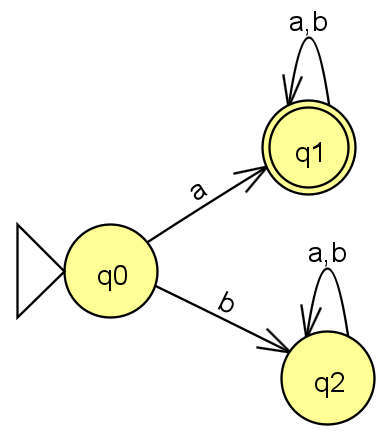
\includegraphics[width=0.2\textwidth]{../../../images/DFAs/ex1_q1.png}



% \vspace{3cm}
% \begin{flushleft}
% أرجو لكم وقتًا ممتعًا.

% الأستاذ محمود اغبارية.
% \end{flushleft}


% \end{document}


\ifwithsols
\title{حل ورقة تمرّن 12 - ترتيب العدّ}
\else
\title{ورقة تمرّن 12 - ترتيب العدّ}
\fi

\begin{document}

\maketitle
\thispagestyle{fancy}

\begin{enumerate}[itemsep=2em]

    % ======================================================
    % 1. GetFrequencies0To16 - مصفوفة تكرار عادية (0-16)
    % ======================================================

    \item
    اكتب عملية خارجية \textenglish{int[] GetFrequencies0To16(int[] arr)} تستقبل مصفوفة أعداد صحيحة، جميع قيمها محصورة في المجال من 0 إلى 16 (شامل). تقوم العملية بإنشاء وإرجاع مصفوفة تكرار (\textenglish{Frequency Array}) تحسب عدد مرات ظهور كل رقم في المصفوفة.

    \begin{boxExample}
    إذا كانت المصفوفة المُدخلة: \textenglish{\{5, 16, 0, 5, 2, 16\}} \\
    فإن العملية تعيد مصفوفة تكرار طولها 17، بحيث تكون:
    \begin{itemize}
        \item قيمة الخانة في الفهرس 5 هي 2 (لأن الرقم 5 ظهر مرتين).
        \item قيمة الخانة في الفهرس 16 هي 2.
        \item قيمة الخانة في الفهرس 0 هي 1.
        \item باقي الخانات قيمتها 0.
    \end{itemize}
    \end{boxExample}

    \ifwithsols
    \begin{boxSolution}
    \begin{english}
    \begin{minted}{csharp}
public static int[] GetFrequencies0To16(int[] arr)
{
    int[] freq = new int[17]; // من 0 إلى 16 يتطلب 17 خانة
    for (int i = 0; i < arr.Length; i++)
    {
        freq[arr[i]]++; // زيادة التكرار في الفهرس المطابق للرقم
    }
    return freq;
}
    \end{minted}
    \end{english}
    \end{boxSolution}
    \clearpage
    \fi

    % ======================================================
    % 2. GetFrequencies5To13 - مصفوفة تكرار مزاحة (5-13)
    % ======================================================

    \item
    اكتب عملية خارجية \textenglish{int[] GetFrequencies5To13(int[] arr)} تستقبل مصفوفة أعداد صحيحة جميع قيمها محصورة في المجال من 5 إلى 13 (شامل). لكي نوفر في مساحة الذاكرة، قم بإنشاء مصفوفة تكرار بأصغر حجم ممكن، وقم بربط كل قيمة بالفهرس المناسب لها.

    \begin{boxHint}
    للحصول على أصغر حجم ممكن، اطرح الحد الأدنى (5) من كل قيمة في المصفوفة. بالتالي، حجم مصفوفة التكرار سيكون $13 - 5 + 1 = 9$.
    \end{boxHint}

    \begin{boxExample}
    إذا كانت المصفوفة المُدخلة: \textenglish{\{5, 13, 8, 5, 10\}} \\
    فإن العملية تعيد مصفوفة تكرار طولها 9، بحيث يكون:
    \begin{itemize}
        \item الفهرس 0 (الذي يمثل الرقم 5) قيمته 2.
        \item الفهرس 8 (الذي يمثل الرقم 13) قيمته 1.
    \end{itemize}
    \end{boxExample}

    \ifwithsols
    \begin{boxSolution}
    \begin{english}
    \begin{minted}{csharp}
public static int[] GetFrequencies5To13(int[] arr)
{
    int[] freq = new int[9]; // الحجم هو 9 خانات
    for (int i = 0; i < arr.Length; i++)
    {
        int index = arr[i] - 5; // طرح 5 للحصول على الفهرس
        freq[index]++;
    }
    return freq;
}
    \end{minted}
    \end{english}
    \end{boxSolution}
    \clearpage
    \fi

    % ======================================================
    % 3. GetEvenFrequencies0To20 - تكرار الأرقام الزوجية
    % ======================================================

    \item
    اكتب عملية خارجية \textenglish{int[] GetEvenFrequencies0To20(int[] arr)} تستقبل مصفوفة أعداد صحيحة تحتوي فقط على أرقام \textbf{زوجية} محصورة في المجال من 0 إلى 20 (شامل). أنشئ مصفوفة تكرار بأصغر حجم ممكن لحساب تكرار هذه الأرقام الزوجية.

    \begin{boxHint}
    بما أن الأرقام المتوقعة هي (0، 2، 4، ... 20)، فإن عددها هو 11 رقماً. يمكنك قسمة كل رقم زوجي على 2 لتحصل على فهرسه المتسلسل في مصفوفة التكرار.
    \end{boxHint}

    \begin{boxExample}
    إذا كانت المصفوفة المُدخلة: \textenglish{\{2, 20, 0, 14, 2\}} \\
    فإن العملية تعيد مصفوفة طولها 11، بحيث يكون:
    \begin{itemize}
        \item الفهرس 1 (الذي يمثل الرقم 2) قيمته 2.
        \item الفهرس 10 (الذي يمثل الرقم 20) قيمته 1.
    \end{itemize}
    \end{boxExample}

    \ifwithsols
    \begin{boxSolution}
    \begin{english}
    \begin{minted}{csharp}
public static int[] GetEvenFrequencies0To20(int[] arr)
{
    int[] freq = new int[11]; // 20 / 2 + 1 = 11
    for (int i = 0; i < arr.Length; i++)
    {
        int index = arr[i] / 2; // القسمة على 2 تعطي الفهرس
        freq[index]++;
    }
    return freq;
}
    \end{minted}
    \end{english}
    \end{boxSolution}
    \clearpage
    \fi

    % ======================================================
    % 4. HasDuplicates - فحص التكرار (استخدام Bool Array)
    % ======================================================

    \item
    اكتب عملية خارجية \textenglish{bool HasDuplicates(int[] arr, int maxVal)} تستقبل مصفوفة أعداد صحيحة جميع قيمها محصورة من 0 إلى \textenglish{maxVal}. تعيد العملية \textenglish{true} إذا وُجد على الأقل رقم واحد مكرر في المصفوفة، وتعيد \textenglish{false} إذا كانت جميع الأرقام مميزة (لا يوجد أي تكرار).

    \begin{boxHint}
    استخدم مصفوفة من نوع \textenglish{bool} لتعقب الأرقام التي مررت عليها سابقاً. إذا صادفت رقماً مسجلاً مسبقاً كـ \textenglish{true}، يمكنك إرجاع الجواب فوراً دون الحاجة لإكمال الفحص.
    \end{boxHint}

    \begin{boxExample}
    \begin{itemize}
        \item إذا كانت المصفوفة: \textenglish{\{1, 5, 3, 9, 5\}} و \textenglish{maxVal = 9}، تعيد العملية \textenglish{true} (لأن الرقم 5 مكرر).
        \item إذا كانت المصفوفة: \textenglish{\{1, 2, 3, 4\}} و \textenglish{maxVal = 5}، تعيد العملية \textenglish{false}.
    \end{itemize}
    \end{boxExample}

    \ifwithsols
    \begin{boxSolution}
    \begin{english}
    \begin{minted}{csharp}
public static bool HasDuplicates(int[] arr, int maxVal)
{
    bool[] seen = new bool[maxVal + 1];
    for (int i = 0; i < arr.Length; i++)
    {
        if (seen[arr[i]] == true) // إذا رأينا الرقم مسبقاً
            return true;

        seen[arr[i]] = true; // نسجل رؤيتنا للرقم
    }
    return false; // إذا انتهت الحلقة ولم نجد تكراراً
}
    \end{minted}
    \end{english}
    \end{boxSolution}
    \fi
    \clearpage

    % ======================================================
    % 5. CountingSort - ترتيب العد
    % ======================================================

    \item
    اكتب عملية خارجية \textenglish{void CountingSort(int[] arr)} تستقبل مصفوفة أعداد صحيحة قيمها محصورة بين 0 و 99. تقوم العملية بترتيب عناصر المصفوفة \textbf{تصاعدياً} باستخدام خوارزمية "ترتيب العد" (\textenglish{Count Sort}).

    \begin{boxHint}
    خوارزمية ترتيب العد تعتمد على خطوتين:
    \begin{enumerate}
        \item بناء مصفوفة التكرار لحساب مرات ظهور كل رقم.
        \item المرور على مصفوفة التكرار واستخدامها لإعادة كتابة الأرقام في المصفوفة الأصلية بشكل مرتب.
    \end{enumerate}
    \end{boxHint}

    \begin{boxExample}
    إذا كانت المصفوفة المُدخلة: \textenglish{\{4, 2, 2, 8, 3, 3, 1\}} \\
    فإنها تصبح بعد استدعاء العملية: \textenglish{\{1, 2, 2, 3, 3, 4, 8\}}.
    \end{boxExample}

    \ifwithsols
    \begin{boxSolution}
    \begin{english}
    \begin{minted}{csharp}
public static void CountingSort(int[] arr)
{
    int[] freq = new int[100]; // مجال الأرقام من 0 إلى 99

    // 1. بناء مصفوفة التكرار
    for (int i = 0; i < arr.Length; i++)
    {
        freq[arr[i]]++;
    }

    // 2. إعادة كتابة المصفوفة الأصلية
    int index = 0;
    for (int i = 0; i < freq.Length; i++)
    {
        while (freq[i] > 0)
        {
            arr[index] = i;
            index++;
            freq[i]--;
        }
    }
}
    \end{minted}
    \end{english}
    \end{boxSolution}
    \clearpage
    \fi

    % ======================================================
    % 6. FindMissingNumber - إيجاد الرقم المفقود
    % ======================================================

    \item
    اكتب عملية خارجية \textenglish{int FindMissingNumber(int[] arr, int n)} تستقبل مصفوفة طولها $n$ تحتوي على أرقام غير مكررة محصورة في المجال من 0 إلى $n$. بما أن طول المصفوفة $n$ والمجال يحتوي على $n+1$ رقماً (من 0 إلى $n$)، فهناك حتماً رقم واحد مفقود. ابحث عن هذا الرقم وأرجعه.

    \begin{boxHint}
    يمكنك استخدام مصفوفة من نوع \textenglish{bool} بحجم $n+1$ لتسجيل الأرقام الموجودة. بعد الانتهاء، الفهرس الوحيد الذي يحمل القيمة \textenglish{false} سيكون هو الرقم المفقود.
    \end{boxHint}

    \begin{boxExample}
    إذا كانت المصفوفة: \textenglish{\{3, 0, 1\}}، وقيمة $n$ هي 3 (أي المجال من 0 إلى 3): \\
    الأرقام التي يجب أن تكون موجودة هي (0، 1، 2، 3). نلاحظ أن الرقم المفقود هو 2، لذا تعيد العملية 2.
    \end{boxExample}

    \ifwithsols
    \begin{boxSolution}
    \begin{english}
    \begin{minted}{csharp}
public static int FindMissingNumber(int[] arr, int n)
{
    bool[] found = new bool[n + 1]; // حجم المصفوفة n+1

    // تسجيل الأرقام الموجودة في المصفوفة
    for (int i = 0; i < arr.Length; i++)
    {
        found[arr[i]] = true;
    }

    // البحث عن الفهرس الذي لم نعثر عليه
    for (int i = 0; i <= n; i++)
    {
        if (found[i] == false)
            return i;
    }

    return -1; // افتراضي في حال لم يتم إيجاد الرقم المفقود
}
    \end{minted}
    \end{english}
    \end{boxSolution}
    \clearpage
    \fi

\end{enumerate}
\end{document}